\chapter{引言}


\section{研究背景}

随着互联网技术的不断发展,社交网络已经成为人们日常生活中不可或缺的一部分,人们可以通过社交网络获取新闻,与他人进行交流互动,发布个人信息等等。对于大多数中国互联网用户来说,QQ、微博、微信、陌陌等社交应用是其日常上网的主要使用应用。根据中国互联网络信息中心(CNNIC)的调查结果显示\cite{internetSurvey},每日的上网时长在两个小时以上的用户达到79.5\%,而其中77.0\%的时间是用在社交应用上。社交网络使得人们不再受报刊、电视等信息来源的限制,拥有了更多获取信息的渠道。

\begin{figure}[h] 
  \centering
  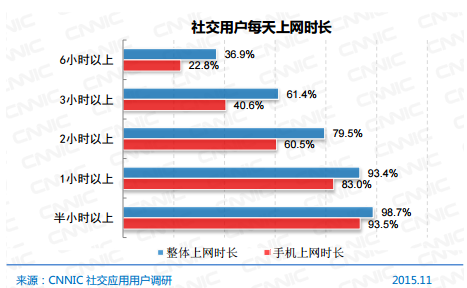
\includegraphics[height=6cm]{InternetUsingTime}
  \caption{社交用户每日上网时长}
  \label{InternetUsingTime}
\end{figure}

对于信息发布者来说,社交网络给他们提供了一个新的推广和营销平台。由于大量用户花费大量时间在社交网络中,传统信息发布渠道日渐衰落,而社交网络凭借其传播范围广、扩散速度快、受众数量大、推广形式多等特点,逐渐成为一种全新的、重要的、高效的推广方式。Shama Hyder在《网络社交媒体营销》一书中提到社交媒体必将取代传统媒介成为营销推广的主要手段 \cite{hyder2016zen}。

利用社交网络进行推广营销,能够在短时间内将信息传递给目标群体。在微博、微信公众号等社交平台上,流行用户往往拥有几百万甚至几千万的关注量,其发布的每一条消息都有大量的用户会关注到。且传播速度快,实时发送接收,还能够根据受众的不同发布不同的信息,使得推广行为更加具有针对性。同时,利用社交网络进行推广,形式上更加灵活多样,文字、图片、语言、视频,能够更加充分进行展示。优秀的推广内容甚至能够通过用户自发进行传播,呈现爆发式营销增长。文献\cite{tuten2014social},\cite{saravanakumar2012social},\cite{heymann2012social},\cite{zavivsic2011social},\cite{bolotaeva2010marketing}均对基于社交网络的营销行为进行了深入分析。著名社交网络公司Facebook,在2016年广告业务的总收入达到268个亿美元\cite{Facebook}。而微博在2016年Q4季度中,其广告收入也达到了1.879亿美元\cite{微博}。而这仅仅是这两家社交网络公司自身的广告营销收入,其最大的贡献是为其用户提供了一个社交网络的营销平台,由此产生的推广营销效益更加巨大。

由于社交网络推广方式的灵活性,包括商品、活动、人物等众多对象均可以进行推广,而本文主要研究的是影视剧在社交网络上的推广。由于影视剧的关注人群广泛,且娱乐性、话题性强,能够更好地适用于社交网络上的多种推广模式。在文献\cite{张琦2011新媒介环境下的中国电影营销策略研究},\cite{于瑞华2012基于},\cite{ono2007context},\cite{golbeck2006filmtrust}中均介绍了基于社交网络数据对影视剧进行推广的研究方法。

随着大数据、机器学习等技术的不断进步,社交网络在影视剧推广方面的重要作用越来越不容忽视。以著名的国产电影《失恋33天》的社交网络营销为例,该部电影在2011年上映,凭借成果的网络营销手段,取得的3.5亿人民币的优秀票房,是愿预估票房的十倍以上\cite{熊莉2012失恋}。在2011年的11月16日,通过百度搜索引擎搜索“失恋33天”关键字,能够找到相关结果约394万个,在谷歌搜索“失恋33天”,能够找到约5900万个相关结果。而在社交网站微博上搜索“失恋33天”能够找到约670万条消息,而在腾讯微博上,则能够搜索到330万条消息\cite{熊莉2012失恋}。

\begin{figure}[h] 
  \centering
  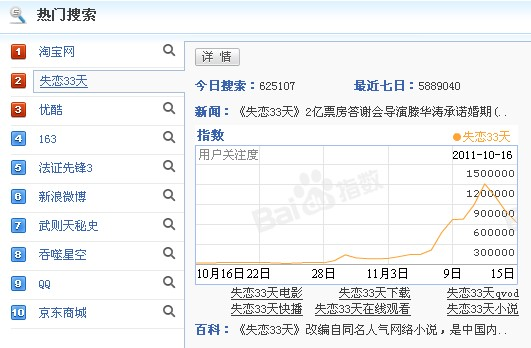
\includegraphics[height=6cm]{失恋}
  \caption{《失恋33天》百度搜索结果}
  \label{失恋}
\end{figure}

这部电影以新浪微博、腾讯微博等社交网站为重要推广平台,打造了拥有近10万粉丝量的官方微博,并创建了众多热门话题,通过宣传短片、制造话题等众多手段,针对网络用户的特点精准投放营销策略,并引导用户参与话题讨论,通过转发、评论等手段,将用户自身的社交网络融入到宣传网络当中,进一步扩大了宣传效果。在日后的各类总结点评中,《失恋33天》都被认为是电影营销手段的一次最成功的创新,利用社交网络对影视剧进行推广的方法从此日益发展。

通过对现有社交网络推广案例进行分析即可发现,目前针对影视剧的网络营销手段层出不穷,而且未来还存在着继续增多的趋势。例如宣传方会在微博、QQ、微信等社交媒体上创建官方账号,发布关于影片的文字、图片消息,演员消息,宣传短片等。这样的宣传方式会在影片上映前后持续较长时间,吸引大量粉丝关注,提高影片关注度。例如最近上映的电影《嫌疑人X的献身》,其在微博上的官方账号共发布了744条微博,拥有62万粉丝关注,发布的每条微博有数千条的转发、评论、点赞\footnote{http://weibo.com/p/1002065746403567}。

\begin{figure}[h] 
  \centering
  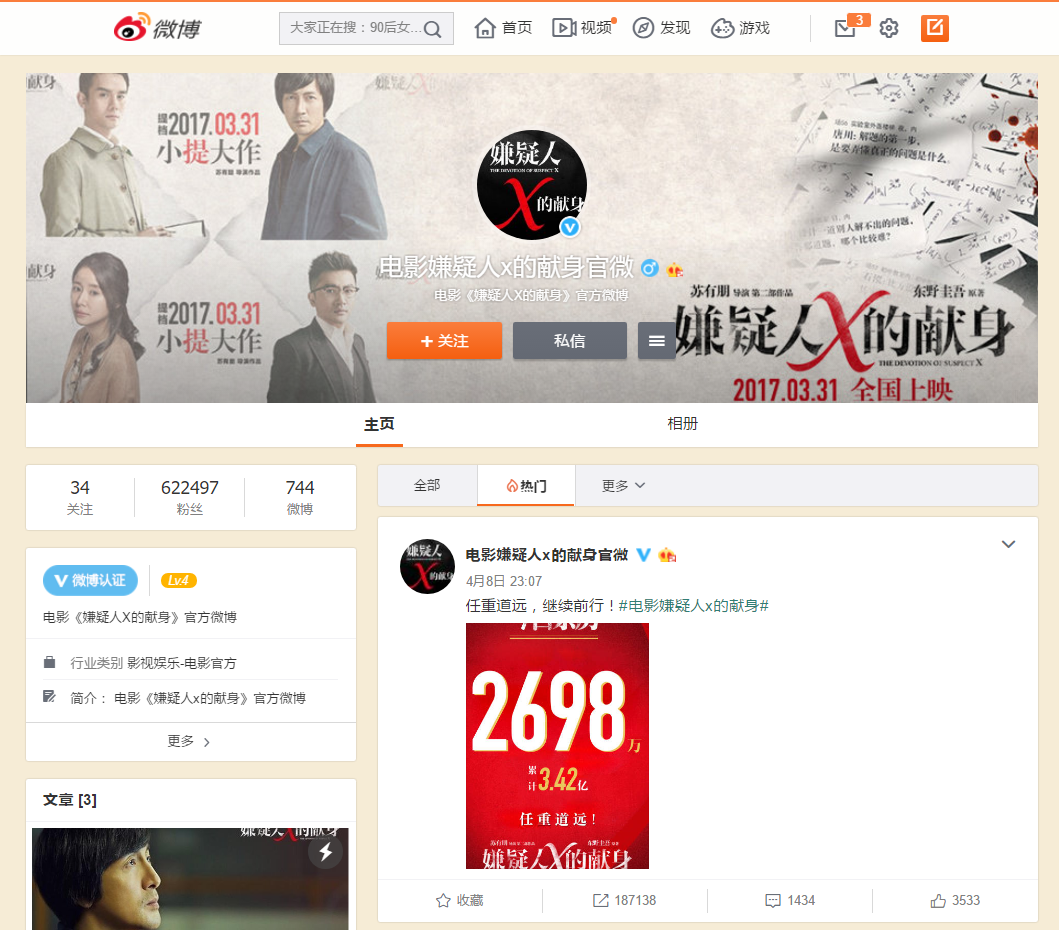
\includegraphics[height=8cm]{嫌疑人}
  \caption{《嫌疑人X的献身》官微截图}
\end{figure}

同时,宣传方还会在社交网络上制造影视剧相关话题,并不断推高话题热度,扩大影片影响力。例如电影《致青春》在网络营销中通过推出“回忆青春”、推出主题曲、制造“有一种感情叫赵薇黄晓明”等流行语等形式制造多个热点话题,激发用户自动传播,最终实现病毒式传播效果。另外宣传方还可以通过各类影评、新闻报道提升观众的观看热情。例如最近热播的电视剧《人民的名义》在豆瓣网可以找到近4万篇影评\footnote{https://movie.douban.com/subject/26727273/},短短一种之内在微信公众号内即出现了55篇与其有关的阅读量超过10万的文章,这样的推广方式能够为影视剧打造良好的口碑,塑造良好形象,吸引更多观众观看。

而网络推广的各种营销手段,往往是通过一些关键节点传播和扩散给广大用户,这些节点一般是由影视剧的官方账号、演员或者经过社交平台验证的“大V”等用户组成。这些用户拥有巨大的粉丝量,能够将各类宣传消息推送给众多的用户,起到宣传媒体的作用\cite{kwak2010twitter}。

影视剧演员往往拥有众多粉丝,关于演员的新闻报道和演员自身发布的消息都能够获得极高的关注度,因此演员在社交网络中也就具有着较高的影响力\cite{shafiq2013identifying},是影视剧宣传推广的重要节点。影视剧演员可以通过自身的影响力在社交网络上制造话题,通过发布各种类型的消息,包括文字、图片、音视频等等,或者利用其它用户发布关于自己的新闻报道,即可以引起关注自己的粉丝的广泛反响,引发相关的热烈讨论。然后根据网络话题演化的规律\cite{he2009detecting},在适当时刻不断推高话题热度,使其成为热点,获得更多受众。因此,在对影视剧进行宣传的过程中,演员就可以利用其巨大的影响力,制造并推动关于影视剧的相关话题,引起其在社交网络中的广泛关注,对影视节目的宣传推广起到重要的促进作用。

但是在进行推广时,不同的推广方式会受到不同的推广效果,同样的推广方式不同的用户使用也会得到不同的结果。如图~\ref{邓超}所示,演员邓超在对其主演的电影《乘风破浪》进行宣传时,发布了两条微博,但是其转发和点赞数量却有很大的不同。可想而知,这两条微博能够获得的推广效果也是截然不同的。

\begin{figure}[h]
  \centering%
  \subcaptionbox{转发:33441 评论:24750 点赞:209791}
    {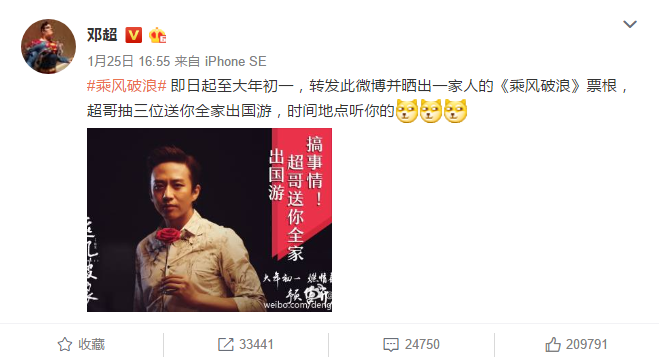
\includegraphics[height=4cm]{邓超1}}
  \subcaptionbox{转发:9327 评论:21477 点赞:560685}
      {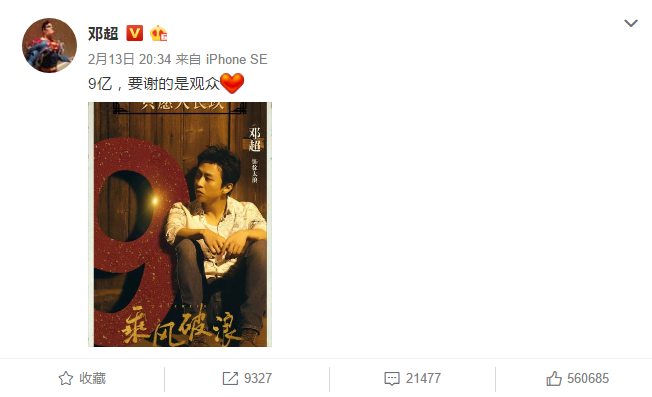
\includegraphics[height=4cm]{邓超2}}
  \caption{不同微博的推广效果比较}
  \label{邓超}
\end{figure}

另外,对于不同的推广对象也需要采取不同的推广策略。例如,对于电影的推广来说,由于其属于一次性消费,只需要吸引观众进入影院观看即可。而对于电视剧的推广来说,由于其播放周期较长,需要对用户存在长时间的粘滞力,在吸引新用户进行观看的同时,还有保持老用户的持续关注。因此,对于电影和电视剧的推广手段就需要有不同的侧重点,需要有针对性地采用不同的推广方式。目前关于电影推广的研究较为常见,由于电影的高投入高产出性,宣传方也会投入更多精力关注电影推广。而关于电视剧有针对性的推广研究较少,推广方式也较为有限,需要给予更多的关注。

因此,为了能够获得更好的推广效果,最大限度地发挥社交网络的推广作用,需要更加具有针对性地为宣传者设计适合其自身特点的推广方式,本文选取演员在社交网络上的对于电视剧的推广行为作为研究对象,针对不同的推广模式进行比较,根据演员自身特点,拍摄混淆变量的干扰,选取最优的推广模式,为演员获得最佳的推广效果提供帮助。

\section{主要研究内容和挑战}

本文主要研究了演员在微博上对电视剧的推广行为,通过倾向值匹配算法分析哪种推广策略能够获得最好的推广效果,从而帮助演员选取适合自己的宣传推广方法,提高电视剧的收视率。

对于电视剧来说社交网络是一个高效的宣传推广平台,越来越多的电视剧宣传方会在微博开设官方账号,发布与电视剧相关的图片、视频等信息以吸引更多的关注。同时,电视剧的各个主要演员,也会在微博个人账号上发布与电视剧相关的信息,宣传自己主演的电视剧。

但是在宣传过程中,有很多的宣传策略可供选择。比如在每天早上发布宣传微博和在晚上发布,获得的评论、点赞数量是不同的。直接转发其他的微博和自己原创一条微博进行推广,获得的关注数量也是不同的。而且相同的推广策略,对于不同的演员和不同的电视剧在使用时,由于其自身特点属性的不同,也会获得不同的效果。因此,本文希望通过分析不同的推广策略与推广效果之间的因果关系,排除其他不相关因素对于推广效果的影响,选出宣传效果最好的推广策略推荐给使用者。

本文获取了爱奇艺、豆瓣和微博这三大社交网站上与电视剧相关的信息数据,和这些电视剧演员在微博上的微博数据,并对这些数据进行了整理分析,从中归纳出了一定的规律,分析出演员在发布微博对电视剧进行推广时,所具有的一些宣传规律。

然后,根据总结出的不同的推广策略,利用倾向值匹配算法逐一分析其与推广效果之间的因果关系。在分析过程中,将其他的相关信息作为混淆变量引入分析模型当中,排除其对于结果的影响,以便更好的比较采用某项推广策略与否对推广效果的影响,从而可以比较出对结果影响最大的推广策略,将其应用在后续的推广过程中,这样就能获得更好的宣传效果。

本文还根据电视剧在微博上的话题演化规律,提出了一种基于话题演化的改进模型,并在倾向值匹配过程中引入更多的混淆变量,排除更多的干扰因素,还对结果进行了模型的显著性及平衡性检验,验证了该方法的适用性和准确性。

本文所述研究主要存在如下几方面挑战:

\begin{itemize}

\item[(1)]目前关于电视剧在社交网络方面的研究较少,关于电视剧在社交网络上的推广行为的研究更是少有相关工作可以参考。对于本文选取的倾向值匹配算法来说,其主要的应用领域为医药学和社会学,分析的数据量往往较小,对于在社交网络领域的大数据应用更是缺乏参考,在实际应用过程当中能否准确分析结果,合理进行应用,还需要进一步的实验验证。

\item[(2)]为了分析出不同的推广策略对于最终推广效果的影响,就需要排除掉其他因素对结果的干扰,而对于电视剧和演员的微博推广来说,能够对推广效果造成影响的因素太多。因此,需要通过因果分析的方法去除其他不相关因素对结果的影响,仅仅针对待分析的推广策略,研究其与推广效果之间的关系。而可以进行因果分析算法有多种,如何从中挑选适合本文研究情境的方法,也是本文的一项调整。

\item[(3)]对于不同的电视剧,不同的演员对其进行推广宣传,由于电视剧和演员自身的特点,各种因素都会对推广效果造成影响,应用相同的推广策略可能会获得不同的推广效果。因此如何针对不同的电视剧和演员,分析出更具针对性的推广策略,个性化定制适合其的推广方法,是本文研究的挑战之一。


\end{itemize}

\section{主要贡献和组织结构}

针对以上提出的问题与挑战,本文利用倾向值匹配算法对演员在微博上发布的推广微博进行了比较分析,对比各个不同策略获得的不同推广效果,找出了适合该演员以及该部电视剧的最优的推广策略。本文的主要贡献如下:

\begin{itemize}

\item[(1)]在以往的研究中,倾向值匹配算法一般多用于医药学和社会科学领域,在大数据及设计媒体领域应用较少,本文将其应用在了对社交媒体数据的分析上,开拓了一种新的应用方向。

\item[(2)]对演员的推广行为进行因果分析,判断各个推广策略对推广效果的直接影响,有效排除了其他非相关变量对结果的干扰,分析结果准确性更高。

\item[(3)]在影视剧研究领域,更多的是对于电影的关注,由于电视剧播出周期长、观看人数少等问题,关于电视剧的研究往往被忽略。而本文选取电视剧为研究对象,分析演员在微博上对其的推广行为,有效填补了对电视剧研究的空白。

\item[(4)]本文利用演员及电视剧官方微博的微博数据作为研究对象,为了避免获取全部微博数据产生的海量数据,本文根据每条微博的内容和话题名称,选取与待推广的电视剧相关的微博进行研究,并提取其中与算法应用相关的信息,有效降低了实验数据量。

\end{itemize}

本文的组织结构如下:

第二章主要介绍当前关于影视剧和社交网络相结合的研究情况,以及因果分析的主要研究方法和基于倾向值匹配的因果分析方法的发展和应用情况。

第三章主要介绍本文所使用的实验数据集,包括数据的来源和收集方法。同时还介绍了关于该数据集的一些基础分析和从中挖掘出的数据特征。

第四章主要介绍了倾向值匹配算法的原理、应用方法以及对分析结果的验证方法。

第五章将前文所介绍的倾向值匹配算法应用到数据集上,对不同的推广策略进行了比较分析,并提出了一种改进模型,验证了该算法对推广策略分析的适用性和准确性。

第六章是对全文的总结,以及对下一步工作的展望。




































